\documentclass[dvipdfmx]{jsarticle}
\usepackage{tikz}
\usepackage{amsmath}
\usepackage{url}
\newcommand{\cat}[1]{\boldsymbol{#1}}
\newcommand{\arrow}{\rightarrow}
\newcommand{\functor}{\rightarrow}
\newcommand{\nat}{\Rightarrow}
\newcommand{\tuple}[1]{\langle #1\rangle}
\newcommand{\obj}[1]{Obj(\cat{#1})}
\newcommand{\mor}[3]{#1:#2\arrow #3}

\newtheorem{proof}{証明}[section]
\newtheorem{prop}{命題}[section]
\newtheorem{define}{定義}[section]
\begin{document}
	\title{圏論入門}
	\maketitle
	\tableofcontents
	\section{はじめに}
	圏論は抽象代数学で生まれ、現在では代数学、幾何学、数学基礎論や、計算機科学、言語学、認知科学、哲学などにも応用されている。
	本資料は数学基礎論や計算機科学で特に使われるデカルト閉圏を中心に解説していく。
	また他の入門書の差別化として、できるだけ議論や具体例を圏論の中で完結するようにしている。
	\section{圏と公理}
	\begin{define}
		ある圏$\cat{C}$は、以下の要素と演算、公理から構成される。
		\begin{itemize}
			\item (1)対象の集合$\obj{C}\ni A,B,C...$
			\item (2)射の集合$Mor(\cat{C})\ni f,g,h...$
			\item (3)射から対象への二つの演算$dom,cod$、もし$dom(f)=A$、$cod(f)=B$であれば、$f\in Mor(A,B)$または$\mor{f}{A}{B}$と表す。
			また、$f$に対する$dom(f)$をドメイン、$cod(f)$をコドメインと呼ぶ。

			ある対象$A,B,C$、ある射$\mor{f}{A}{B}$、$\mor{g}{A}{C}$、$\mor{h}{C}{B}$について考えるとき、以下のような図式を用いて議論を行うことがある。
			\begin{center}
				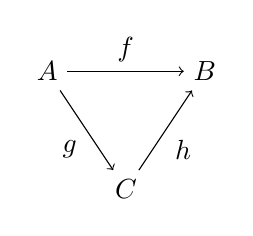
\begin{tikzpicture}[auto]
					\node (a) at (0, 0) {$A$};
					\node (b) at (2, 0) {$B$};
					\node (c) at (1, -1.5) {$C$};
					\draw[->] (a) to node {$f$}(b);
					\draw[->] (a) to node[swap] {$g$}(c);
					\draw[->] (c) to node[swap] {$h$}(b);
				\end{tikzpicture}
			\end{center}

			\item (4)ある射$f,g$が$cod(f)=dom(g)$を満たす、つまり$\mor{f}{X}{A}$、$\mor{g}{A}{Y}$であるようなとき、射の合成$\mor{g\circ f}{X}{Y}$が行える。
			射をつなげる、という直感に反して合成射の射の順序が射の向きと逆であることに注意すべきである。

			射$h,g$の合成$h\circ g$は次のように表せる。
			また対象$A$と対象$B$の間の射は一つとは限らないので、必ずしも$h\circ g=f$が成り立つわけではない。
			\begin{center}
				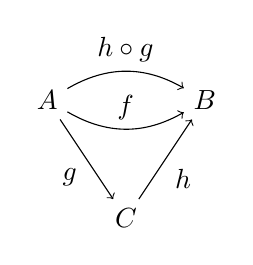
\begin{tikzpicture}[auto]
					\node (a) at (0, 0) {$A$};
					\node (b) at (2, 0) {$B$};
					\node (c) at (1, -1.5) {$C$};
					\draw[->] (a) to[bend right=30] node {$f$}(b);
					\draw[->] (a) to[bend right=-30] node {$h\circ g$}(b);
					\draw[->] (a) to node[swap] {$g$}(c);
					\draw[->] (c) to node[swap] {$h$}(b);
				\end{tikzpicture}
			\end{center}
			\item (5)恒等射と呼ばれる特別な射$\mor{id_A}{A}{A}$が任意の対象に存在する。
			\item (6)結合則$h\circ (g\circ f)=(h\circ g)\circ f$が合成可能な任意の射$f,g,h$で成り立つ。

				\begin{center}
				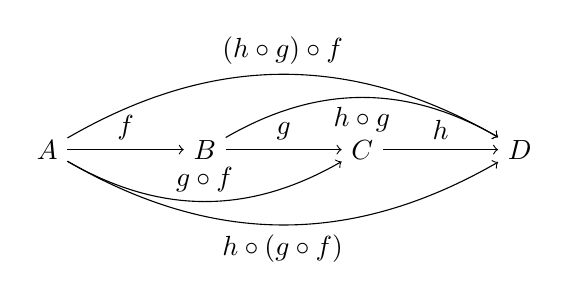
\begin{tikzpicture}[auto]
					\node (a) at (0, 0) {$A$};
					\node (b) at (2, 0) {$B$};
					\node (c) at (4, 0) {$C$};
					\node (d) at (6, 0) {$D$};
					\draw[->] (a) to node {$f$}(b);
					\draw[->] (b) to node {$g$}(c);
					\draw[->] (c) to node {$h$}(d);
					\draw[->] (a) to[bend right=30] node {$g\circ f$}(c);
					\draw[->] (a) to[bend right=30] node[swap] {$h\circ(g\circ f)$}(d);
					\draw[->] (b) to[bend left=30] node[swap] {$h\circ g$}(d);
					\draw[->] (a) to[bend left=30] node {$(h\circ g)\circ f$}(d);
				\end{tikzpicture}
			\end{center}
			\item (7)任意の対象$A$と対応する恒等射$\mor{id_A}{A}{A}$、任意の射$\mor{f}{X}{A}$、$\mor{g}{A}{Y}$において$id_A\circ f=f$、$g\circ id_A=g$が成り立つ。

			恒等射をある射に合成しても、合成する前の射と等しくなることから、直感的に恒等射は何も行わない射のように考えられる。

			\begin{center}
				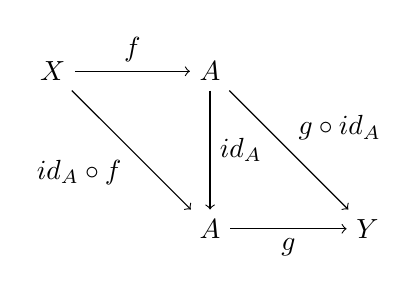
\begin{tikzpicture}[auto]
					\node (a) at (0, 0) {$X$};
					\node (b) at (2, 0) {$A$};
					\node (b') at (2, -2) {$A$};
					\node (c) at (4, -2) {$Y$};
					\draw[->] (a) to node {$f$}(b);
					\draw[->] (b) to node {$id_A$}(b');
					\draw[->] (b') to node[swap]  {$g$}(c);
					\draw[->] (a) to node[swap]  {$id_A\circ f$}(b');
					\draw[->] (b) to node {$g\circ id_A$}(c);
				\end{tikzpicture}
			\end{center}
		\end{itemize}
	\end{define}

	%\subsection{前順序圏}
	%前順序集合は反射律と推移律を満たす順序集合である。
	%この前順序集合$P$の元を対象、ある元$a,b$の間の順序関係$a\leq b$を$a$から$b$への射とする圏を$\cat{Pre}$とすると、反%射律より恒等射の存在が、推移律より射の結合則が満たされる。

	%圏$\cat{Pre}$では任意の二対象の間の射が高々一つしかない。
	%そのため、恒等射の性質や結合則に現れる等式は必ず成り立つ。
	次に圏の具体例としてスライス圏と呼ばれる圏を定義する。
	%\begin{define}[スライス圏]
	%	圏$\cat{C}$と$\cat{C}$のある対象$A$に対するスライス圏$\cat{C}/A$は以下のように定義する。
	%	\begin{itemize}
	%		\item (1)
	%		$\cat{C}$の
	%		\item (2)
	%		$\cat{C}/A$の対象である$\mor{f}{A}{X}$と$\mor{g}{B}{X}$に対して射$\mor{h}{A}{B}$が存在し、$g\circ h=g$が成り立つとき、射$h$を$\cat{C}/A$の射$\mor{s_h}{S_f}{S_g}$とする。
	%		\item (3)
	%	\end{itemize}

	%\end{define}
	\section{圏論の基本概念}
	まずはこれまで図示してきた図式について数学的な定義を与える。
	\begin{define}[図式(部分圏)]
		ある圏$\cat{C}$のある図式(部分圏)とは、圏$\cat{C}$に含まれるいくつかの対象と、いくつかの射で構成される圏であり、任意の対象に対応する恒等射を含み、図式中の任意の合成可能な二射$\mor{f}{X}{Y},\mor{g}{Y}{Z}$が含まれるとき、その合成射$g\circ f$も含むような圏である。
	\end{define}
	また図式は単に図示するために使用する以外にも、圏論のいくつかの概念を定義するのにも用いられる。
	\begin{define}[可換]
		圏におけるいくつかの射と対象の集まりである図式が可換である。すなわち可換図式であるとは、図式中の対象を頂点、図式中の射を辺とする有向グラフを考えたとき、任意の頂点$C,C'$において$C$から$C'$への任意の経路によって表される射が等しいときである。
	\end{define}
	例えば以下の図式において$j\circ g=l\circ i,k\circ h=m\circ j,k\circ h\circ g=m\circ j\circ g = m\circ l\circ i$が成り立つとすると、これは可換図式になる。

	\begin{center}
		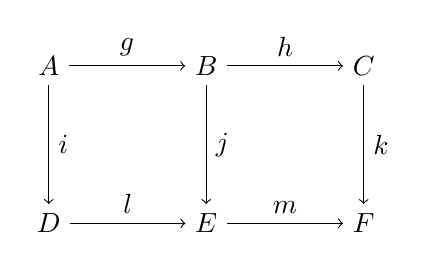
\begin{tikzpicture}[auto]
			\node (a) at (0, 0) {$A$};
			\node (b) at (2, 0) {$B$};
			\node (c) at (4, 0) {$C$};
			\node (d) at (0, -2) {$D$};
			\node (e) at (2, -2) {$E$};
			\node (f) at (4, -2) {$F$};
			\draw[->] (a) to node {$g$}(b);
			\draw[->] (b) to node {$h$}(c);
			\draw[->] (a) to node {$i$}(d);
			\draw[->] (b) to node {$j$}(e);
			\draw[->] (c) to node {$k$}(f);
			\draw[->] (d) to node {$l$}(e);
			\draw[->] (e) to node {$m$}(f);
		\end{tikzpicture}
	\end{center}
	\subsection{同型}
	\begin{define}[同型]
		ある対象$A$と$B$が同型、つまり$A\cong B$であるとは、$f\circ f^{-1}=id_B$と$f^{-1}\circ f=id_A$を満たすようなある二つの射$\mor{f}{A}{B}$とその逆射$\mor{f^{-1}}{B}{A}$が存在するときである。
		また、このような射$f,f^{-1}$を同型射と呼ぶ。
	\end{define}
	\begin{center}
		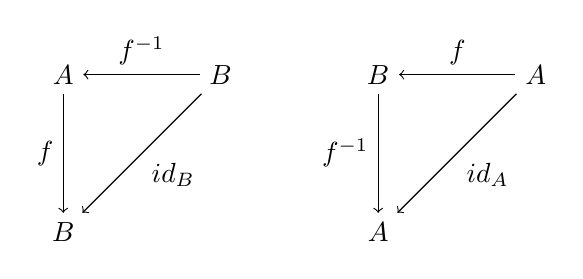
\begin{tikzpicture}[auto]
			\node (a) at (0, 0) {$A$};
			\node (b) at (2, 0) {$B$};
			\node (b') at (0, -2) {$B$};
			\draw[->] (a) to node[swap] {$f$}(b');
			\draw[->] (b) to node {$id_B$}(b');
			\draw[->] (b) to node[swap] {$f^{-1}$}(a);

			\node (a) at (4, 0) {$B$};
			\node (b) at (6, 0) {$A$};
			\node (b') at (4, -2) {$A$};
			\draw[->] (a) to node[swap] {$f^{-1}$}(b');
			\draw[->] (b) to node {$id_A$}(b');
			\draw[->] (b) to node[swap] {$f$}(a);
		\end{tikzpicture}
	\end{center}
	圏論での同型は直感的には二つの対象の持つ振る舞いが一致するような同値関係として扱われる。
	これを圏論の言葉で記述する。
	\begin{prop}
		$A\cong A' \Longleftrightarrow$任意の対象$X$、任意の射$\mor{f}{A}{X}$に対してある射$\mor{f'}{A'}{X}$が存在して、$A\cong A'$の同型射を$i,i^{-1}$とすると$f'\circ i=f$、$f\circ i^{-1}=f'$が成り立つ。
		\begin{center}
			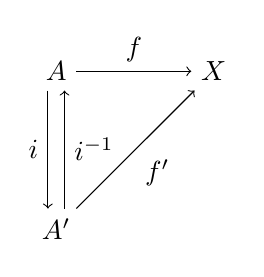
\begin{tikzpicture}[auto]
				\node (a) at (0, 0) {$A$};
				\node (a') at (0, -2) {$A'$};
				\node (x) at (2, 0) {$X$};
				\draw[->,transform canvas={xshift=-3pt}] (a) to node[swap] {$i$}(a');
				\draw[->,transform canvas={xshift=3pt}] (a') to node[swap] {$i^{-1}$}(a);
				\draw[->] (a) to node {$f$}(x);
				\draw[->] (a') to node[swap] {$f'$}(x);
			\end{tikzpicture}
		\end{center}
	\end{prop}

	$A$と$A'$の間にある相互変換となる射である同型射$\mor{i}{A}{A'}$、$\mor{i^{-1}}{A'}{A}$が存在して、$A$と$A'$の振る舞いとして任意の$X$と任意の射$\mor{f}{A}{X}$とそれに対応する$\mor{f'}{A'}{X}$を考える。
	もし、$A$と$A'$の振る舞いが一致するならば、$f$とある変換$i$を経由した$f'$、つまり$f'\circ i$が等しくなり、同様に$f'$とある変換$i^{-1}$を経由した$f$、つまり$f\circ i^{-1}$が等しくなるはずである。

	\begin{proof}
		$(\Longleftarrow)$ $f=f'\circ i$、$f'=f\circ i^{-1}$にそれぞれもう一方をお互いに代入することで$f'\circ i\circ i^{-1}=f'$、$f\circ i^{-1}\circ i=f$が成り立つ。これらは$i,i^{-1}$に対して任意の$X,f$について成り立つから、$X,f$に$A,id_A$と$A',id_A'$を当てはめると、それぞれ$i\circ i^{-1}=id_A$、$i^{-1}\circ i=id_A'$が成り立つ。

		\begin{center}
			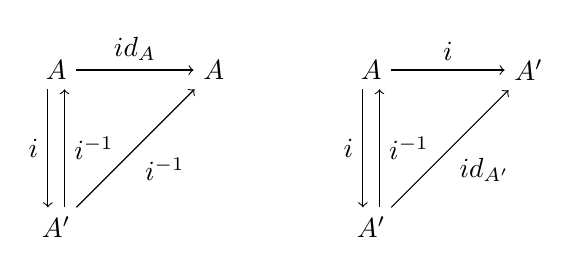
\begin{tikzpicture}[auto]
				\node (a) at (0, 0) {$A$};
				\node (a') at (0, -2) {$A'$};
				\node (x) at (2, 0) {$A$};
				\draw[->,transform canvas={xshift=-3pt}] (a) to node[swap] {$i$}(a');
				\draw[->,transform canvas={xshift=3pt}] (a') to node[swap] {$i^{-1}$}(a);
				\draw[->] (a) to node {$id_A$}(x);
				\draw[->] (a') to node[swap] {$i^{-1}$}(x);

				\node (a2) at (4, 0) {$A$};
				\node (a'2) at (4, -2) {$A'$};
				\node (x2) at (6, 0) {$A'$};
				\draw[->,transform canvas={xshift=-3pt}] (a2) to node[swap] {$i$}(a'2);
				\draw[->,transform canvas={xshift=3pt}] (a'2) to node[swap] {$i^{-1}$}(a2);
				\draw[->] (a2) to node {$i$}(x2);
				\draw[->] (a'2) to node[swap] {$id_{A'}$}(x2);
			\end{tikzpicture}
		\end{center}


		$(\Longrightarrow)$ 任意の対象$X$と射$\mor{f}{A}{X}$に対して$f$に対応する射$f'$を$f\circ i^{-1}$とすると、$f'=f\circ i^{-1}$となり、両辺に$i$を合成して$f'\circ i=f\circ i^{-1}\circ i$となり、$A\cong A'$の定義より$f'\circ i=f$。よって求められる条件を満たした$f'$の存在を示せた。とう
	\end{proof}


	今回は$A\cong A'$とそれらから伸びる射$\mor{f}{A}{X}$、$\mor{f'}{A'}{X}$の関係性を見たが、$A\cong A'$とそれらへ伸びる射$\mor{g}{Y}{A}$、$\mor{g'}{Y}{A'}$の関係においても同様に成り立つ。
	\subsection{元}
	集合論では集合から集合への関数の性質を述べるのに集合の元を用いることが多いが、圏の対象では一般的に元を取ることができない。
	しかしある圏$\cat{C}$に終対象$1$と呼ばれる特別な対象が存在するとき、$\cat{C}$の任意の対象$A$のある元(global elements)はある射$\mor{a}{1}{A}$で表せる。
	\begin{center}
		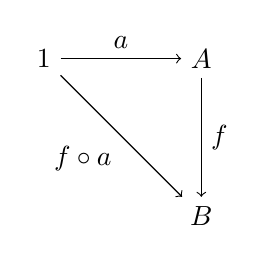
\begin{tikzpicture}[auto]
			\node (a) at (2, 0) {$A$};
			\node (b) at (2, -2) {$B$};
			\node (1) at (0, 0) {$1$};
			\draw[->] (1) to node {$a$}(a);
			\draw[->] (1) to node[swap] {$f\circ a$}(b);
			\draw[->] (a) to node {$f$}(b);
		\end{tikzpicture}
	\end{center}

	射$\mor{f}{A}{B}$に対して$\mor{a}{1}{A}$を適用する操作は、そのまま関数の合成$\mor{f\circ a}{1}{B}$で表せる。
	射を適用した元もまた終対象からの射になるから$f\circ a$もまた対象$B$の元になる。
	終対象の定義や、ある対象と終対象からその対象への射の全体が等価になることについては、当分先になるであろうが後に説明する。
	これから説明する圏論の概念たちの解説に使用するためここで軽く説明した。
	\subsection{演習問題}
	\begin{enumerate}
		\item 以下の図式において左側の正方形の図式と右側の正方形の図式がそれぞれ可換になるとき、二つを合わせた長方形の図式が可換になることを示せ。
			\begin{center}
				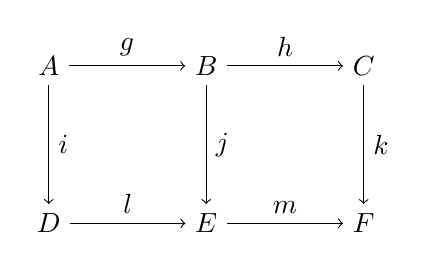
\begin{tikzpicture}[auto]
					\node (a) at (0, 0) {$A$};
					\node (b) at (2, 0) {$B$};
					\node (c) at (4, 0) {$C$};
					\node (d) at (0, -2) {$D$};
					\node (e) at (2, -2) {$E$};
					\node (f) at (4, -2) {$F$};
					\draw[->] (a) to node {$g$}(b);
					\draw[->] (b) to node {$h$}(c);
					\draw[->] (a) to node {$i$}(d);
					\draw[->] (b) to node {$j$}(e);
					\draw[->] (c) to node {$k$}(f);
					\draw[->] (d) to node {$l$}(e);
					\draw[->] (e) to node {$m$}(f);
				\end{tikzpicture}
				\begin{tikzpicture}[auto]
					\node (a) at (4, 0) {$A$};
					\node (c) at (8, 0) {$C$};
					\node (d) at (4, -2) {$D$};
					\node (f) at (8, -2) {$F$};
					\draw[->] (a) to node {$h\circ g$}(c);
					\draw[->] (d) to node {$m\circ l$}(f);
					\draw[->] (a) to node {$i$}(d);
					\draw[->] (c) to node {$k$}(f);
				\end{tikzpicture}
			\end{center}
		\item $A\cong B$かつ$B\cong C$ならば$A\cong C$であることを示せ。
	\end{enumerate}

	\section{普遍性}
	普遍性はある対象と射を特徴づけるために使用される。
	この段階で普遍性を用いた各概念を一般化することはできないが、この章で扱う普遍性に限定して一般化する。
	\begin{itemize}
		\item (1) ある圏$\cat{C}$のある図式$\cat{D}$が存在する。

		また例として、以下の図式における普遍性を考える。
		\begin{center}
			\begin{tikzpicture}[auto]
				\node (i) at (0, 0) {$I$};
				\node (j) at (2, 0) {$J$};
				\draw[->] (i) to node {$k$}(j);
			\end{tikzpicture}
		\end{center}
		\item (2) (1)の図式$\cat{D}$に対して圏$\cat{C}$のある対象$U$と、$U$から図式$D$の任意の対象$A$に対してある射$\mor{\tau_A}{U}{A}$が存在する。

		また対象$U$と任意の対象$A$に存在する射の全体を対として$(U,(\mor{\tau_A}{U}{A})_{A\in D})$と表す。
		\begin{center}
			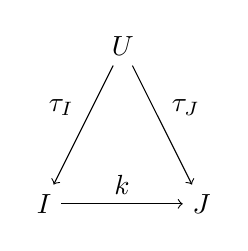
\begin{tikzpicture}[auto]
				\node (i) at (0, 0) {$I$};
				\node (j) at (2, 0) {$J$};
				\node (u) at (1, 2) {$U$};
				\draw[->] (i) to node {$k$}(j);
				\draw[->] (u) to node[swap] {$\tau_I$}(i);
				\draw[->] (u) to node {$\tau_J$}(j);
			\end{tikzpicture}
		\end{center}
		\item (3)図式$\cat{D}$と対$(U,(\tau_A)_{A\in D})$を合わせた図式が可換になる。

		すなわち、図式$\cat{D}$の任意の射$\mor{f}{A}{B}$と$\mor{\tau_A}{U}{A}$の合成$\mor{f\circ\tau_A}{U}{B}$が$\mor{\tau_B}{U}{B}$と等しくなる。

		今考えている図式で表すなら$f\circ\tau_I=\tau_J$となる。
		\item (4)
		(2)と(3)を同様に満たすようなまた別の対$(X,(\mor{\phi_A}{X}{A})_{A\in D})$が存在するとき、ある射$\mor{u}{X}{U}$が存在する。
		\begin{center}
			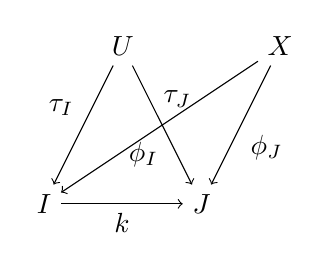
\begin{tikzpicture}[auto]
				\node (i) at (0, 0) {$I$};
				\node (j) at (2, 0) {$J$};
				\node (u) at (1, 2) {$U$};
				\node (x) at (3, 2) {$X$};
				\draw[->] (i) to node[swap] {$k$}(j);
				\draw[->] (u) to node[swap] {$\tau_I$}(i);
				\draw[->] (u) to node[transform canvas={xshift=-3pt,yshift=3pt}] {$\tau_J$}(j);
				\draw[->] (x) to node[swap,transform canvas={xshift=3pt,yshift=-18pt}] {$\phi_I$}(i);
				\draw[->] (x) to node {$\phi_J$}(j);
			\end{tikzpicture}
			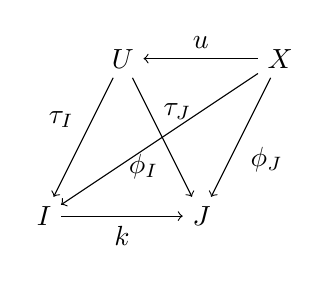
\begin{tikzpicture}[auto]
				\node (i) at (0, 0) {$I$};
				\node (j) at (2, 0) {$J$};
				\node (u) at (1, 2) {$U$};
				\node (x) at (3, 2) {$X$};
				\draw[->] (i) to node[swap] {$k$}(j);
				\draw[->] (x) to node[swap] {$u$}(u);
				\draw[->] (u) to node[swap] {$\tau_I$}(i);
				\draw[->] (u) to node[transform canvas={xshift=-3pt,yshift=3pt}] {$\tau_J$}(j);
				\draw[->] (x) to node[swap,transform canvas={xshift=3pt,yshift=-18pt}] {$\phi_I$}(i);
				\draw[->] (x) to node {$\phi_J$}(j);
			\end{tikzpicture}
		\end{center}
		\item (5)
		(4)図式$\cat{D}$と二つの対$(U,(\tau_A)_{A\in D})$、$(X,(\phi_A)_{A\in D})$を合わせた図式に対して、射$\mor{u}{X}{U}$はこの図式を可換にし、このような射は一意に定まる。

		すなわち、図式$\cat{D}$の任意の対象$A$において、$\tau_A\circ u =\phi_A$が成り立つ。
	\end{itemize}

	\subsection{積}
	\begin{define}

		積$A\times B$と二つの射$\mor{\pi_A}{A\times B}{A}$、$\mor{\pi_B}{A\times B}{B}$がある二対象$A,B$における積であるとは、ある対象$X$と二つの射$\mor{f}{X}{A}$、$\mor{g}{X}{B}$が存在するとき、図を可換にする、つまり$\pi_A\circ\tuple{f,g}=f$、$\pi_B\circ\tuple{f,g}=g$が成り立つような$\tuple{f,g}$が一意に存在する。
		また$\pi_A$、$\pi_B$を射影射、$\tuple{f,g}$を$f$と$g$の対と呼ぶ。
		ある圏$\cat{C}$の任意の二対象に対して積が存在するとき、圏$\cat{C}$は積を持つという。

		\begin{center}
			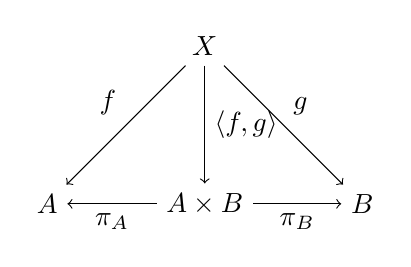
\begin{tikzpicture}[auto]
				\node (a) at (0, 0) {$A$};
				\node (b) at (4, 0) {$B$};
				\node (ab) at (2, 0) {$A\times B$};
				\node (x) at (2, 2) {$X$};
				\draw[->] (ab) to node {$\pi_A$}(a);
				\draw[->] (ab) to node[swap] {$\pi_B$}(b);
				\draw[->] (x) to node[swap] {$f$}(a);
				\draw[->] (x) to node {$g$}(b);
				\draw[->] (x) to node {$\tuple{f,g}$}(ab);
			\end{tikzpicture}
		\end{center}
	\end{define}

	つまり、ある射$\mor{h}{X}{A\times B}$が存在して$\pi_A\circ h=f$、$\pi_B\circ h=g$を満たすとき、このような射は一意に存在するから$h=\tuple{f,g}$となる。

	上の定義を普遍性の一般化に基づいて改めて定義すると、
	\begin{itemize}
		\item (1)
		図式$\cat{D}$として、二つの対象$A,B$、それぞれの恒等射$id_A$、$id_B$で構成される図式を考える。
		\item (2)対$(U,(\tau_A)_{A\in D})$を$(A\times B,\{\pi_A,\pi_B\})$として考える。
		\item (3)
		今回は図式に含まれる射が恒等射のみであるため、可換性が無条件に成り立つ。
		\item (4)
		任意の対象$X$の射から、$A,B$への射をそれぞれ$\mor{f}{X}{A}$、$\mor{g}{X}{B}$とする。
		対$(X,(\phi_A)_{A\in D})$を$(X,\{f,g\})$として考える。
		そして射$u$を$\tuple{f,g}$とする。
		\item (5)
		これらの図式が可換になる、つまり$\pi_A\circ\tuple{f,g}=f$、$\pi_B\circ\tuple{f,g}=g$が成り立つような射$\tuple{f,g}$が一意に定まる。
	\end{itemize}

	ここで$X$に終対象$1$を当てはめると、$A$のある元$a$、$B$のある元$b$に対して$\pi_A\circ\tuple{a,b}=a$、$\pi_B\circ\tuple{a,b}=b$が成り立つような$\tuple{a,b}$が一意に定まる。
	直感的には$\pi_A$と$\pi_B$は$A\times B$の元$\tuple{a,b}$からそれぞれ$A$の元と$B$の元を取りだす。もし$A\times B$のまた別の元$\mor{h}{1}{A\times B}$からも$a$と$b$が取り出せたなら、$h=\tuple{a,b}$となることがわかる。

	\begin{center}
		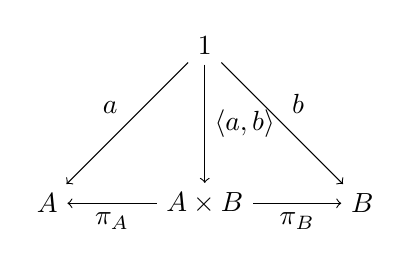
\begin{tikzpicture}[auto]
			\node (a) at (0, 0) {$A$};
			\node (b) at (4, 0) {$B$};
			\node (ab) at (2, 0) {$A\times B$};
			\node (x) at (2, 2) {$1$};
			\draw[->] (ab) to node {$\pi_A$}(a);
			\draw[->] (ab) to node[swap] {$\pi_B$}(b);
			\draw[->] (x) to node[swap] {$a$}(a);
			\draw[->] (x) to node {$b$}(b);
			\draw[->] (x) to node {$\tuple{a,b}$}(ab);
		\end{tikzpicture}
	\end{center}

	次に積の性質をいくつか見ていく。
	\begin{prop}[射の対の分配則]
		$\mor{f}{X}{A}$、$\mor{g}{X}{B}$、$\mor{h}{Y}{X}$に対して$\tuple{f,g}\circ h=\tuple{f\circ h,g\circ h}$が成り立つ
	\end{prop}
	\begin{proof}
		積$A\times B$に対し、(4)の対$(X,\{f,g\})$に$(Y,\{f\circ h, g\circ h\})$を当てはめると、(5)よりこの図式を可換にする対象と射の対$\mor{\tuple{f\circ h,g\circ h}}{Y}{A\times B}$が存在し一意に定まる。
		よって$\tuple{f,g}\circ h=\tuple{f\circ h,g\circ h}$が成り立つ。
	\end{proof}

	\begin{center}
		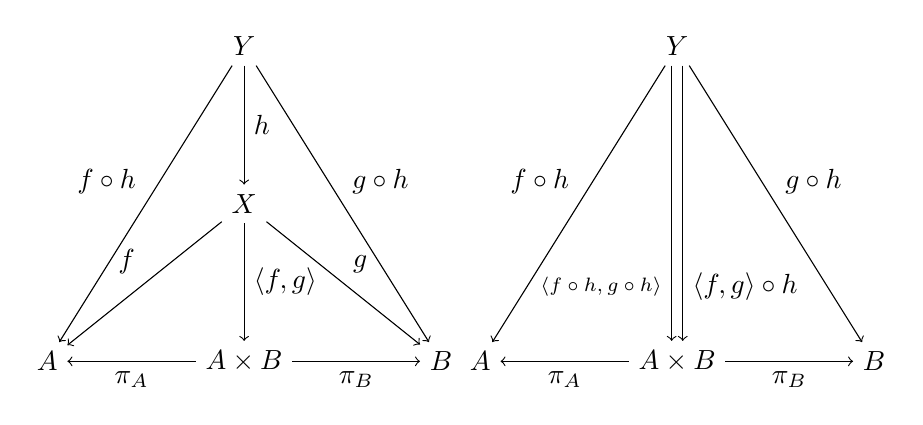
\begin{tikzpicture}[auto]
			\node (y) at (3, 4) {$Y$};
			\node (a) at (0.5, 0) {$A$};
			\node (b) at (5.5, 0) {$B$};
			\node (ab) at (3, 0) {$A\times B$};
			\node (x) at (3, 2) {$X$};
			\draw[->] (y) to node {$h$}(x);
			\draw[->] (y) to node[swap] {$f\circ h$}(a);
			\draw[->] (y) to node {$g\circ h$}(b);
			\draw[->] (ab) to node {$\pi_A$}(a);
			\draw[->] (ab) to node[swap] {$\pi_B$}(b);
			\draw[->] (x) to node[swap] {$f$}(a);
			\draw[->] (x) to node {$g$}(b);
			\draw[->] (x) to node {$\tuple{f,g}$}(ab);

			\node (y) at (8.5, 4) {$Y$};
			\node (a) at (6, 0) {$A$};
			\node (b) at (11, 0) {$B$};
			\node (ab) at (8.5, 0) {$A\times B$};
			\draw[->, transform canvas={xshift=2pt}] (y) to node[yshift=-30pt] {$\tuple{f,g}\circ h$}(ab);
			\draw[->, transform canvas={xshift=-2pt}] (y) to node[yshift=-30pt, swap] {\scriptsize{$\tuple{f\circ h,g\circ h}$}}(ab);
			\draw[->] (y) to node[swap] {$f\circ h$}(a);
			\draw[->] (y) to node {$g\circ h$}(b);
			\draw[->] (ab) to node {$\pi_A$}(a);
			\draw[->] (ab) to node[swap] {$\pi_B$}(b);
		\end{tikzpicture}
	\end{center}
	$y$を終対象、$h$を元とすれば射の対がどのような操作かがわかるだろう。

	次に、任意の積から任意の積への射である、射の積を定義していく。
	二つの対象から二つの対象へ射を一つの射に纏めることから、直感的に射の積は並列処理のように思える。
	\begin{define}[射の積]
		射$\mor{f}{A}{A'}$、$\mor{g}{B}{B'}$に対して射の積$\mor{f\times g}{A\times B}{A'\times B'}$を$f\times g = \tuple{f\circ\pi_A,g\circ\pi_B}$と定義する。
		\begin{center}
			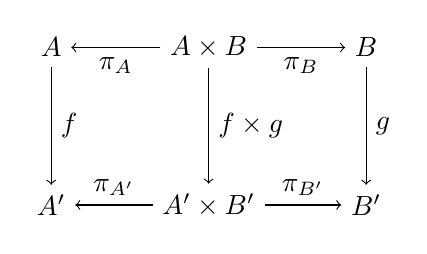
\begin{tikzpicture}[auto]
				\node (a) at (0, 0) {$A$};
				\node (ab) at (2, 0) {$A\times B$};
				\node (b) at (4, 0) {$B$};
				\node (a') at (0, -2) {$A'$};
				\node (a'b') at (2, -2) {$A'\times B'$};
				\node (b') at (4, -2) {$B'$};
				\draw[->] (a'b') to node[swap] {$\pi_{A'}$}(a');
				\draw[->] (a'b') to node {$\pi_{B'}$}(b');
				\draw[->] (ab) to node {$\pi_A$}(a);
				\draw[->] (ab) to node[swap] {$\pi_B$}(b);
				\draw[->] (a) to node {$f$}(a');
				\draw[->] (b) to node {$g$}(b');
				\draw[->] (ab) to node {$f\times g$}(a'b');
			\end{tikzpicture}
		\end{center}
	\end{define}
	射の対は任意の対象から任意の積への射であるのに対し、射の積は任意の積から任意の積への射である。


	\begin{prop}[積と合成の交換]
		射の積$\mor{f\times g}{A\times B}{A'\times B'}$、$\mor{f'\times g'}{A'\times B'}{A''\times B''}$に対して、$(f'\times g')\circ(f\times g)=(f'\circ f)\times(g'\circ g)$が成り立つ。
	\end{prop}
	\begin{proof}
		上の図式と下の図式はそれぞれ射の積の図式であり可換であるため、図式全体も可換になる。

		また積$A''\times B''$において、(4)の対$(X,\{f,g\})$に$(A\times B,\{f'\circ f\circ\pi_A$と$g'\circ g\circ\pi_B\})$を当てはめると射$\mor{\tuple{f'\circ f\circ\pi_A,g'\circ g\circ\pi_B}}{A\times B}{A''\times B''}$が存在する。

		また射の積の定義より、$\tuple{f'\circ f\circ\pi_A,g'\circ g\circ\pi_B}=(f'\circ f)\times(g'\circ g)$が成り立つ。

		ここで図式全体が可換になるため、$(f'\times g')\circ(f\times g)$も同様に積の図式を可換にする。よって、射の一意性より、$(f'\times g')\circ(f\times g)=(f'\circ f)\times(g'\circ g)$が成り立つ。
		\begin{center}
			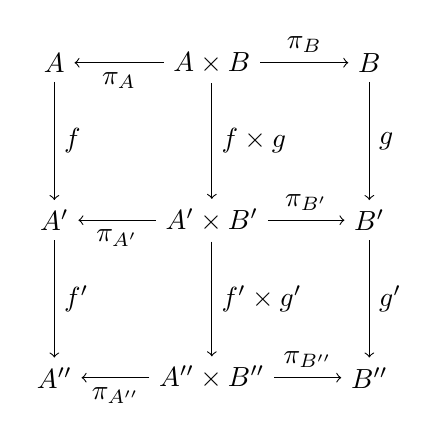
\begin{tikzpicture}[auto]
				\node (a) at (0, 0) {$A$};
				\node (a') at (0, -2) {$A'$};
				\node (a'') at (0, -4) {$A''$};
				\node (ab) at (2, 0) {$A\times B$};
				\node (ab') at (2, -2) {$A'\times B'$};
				\node (ab'') at (2, -4) {$A''\times B''$};
				\node (b) at (4, 0) {$B$};
				\node (b') at (4, -2) {$B'$};
				\node (b'') at (4, -4) {$B''$};
				\draw[->] (ab) to node{$\pi_{A}$}(a);
				\draw[->] (ab) to node{$\pi_{B}$}(b);
				\draw[->] (ab') to node{$\pi_{A'}$}(a');
				\draw[->] (ab') to node{$\pi_{B'}$}(b');
				\draw[->] (ab'') to node{$\pi_{A''}$}(a'');
				\draw[->] (ab'') to node{$\pi_{B''}$}(b'');
				\draw[->] (a) to node{$f$}(a');
				\draw[->] (a') to node{$f'$}(a'');
				\draw[->] (b) to node{$g$}(b');
				\draw[->] (b') to node{$g'$}(b'');
				\draw[->] (ab) to node{$f\times g$}(ab');
				\draw[->] (ab') to node{$f'\times g'$}(ab'');
			\end{tikzpicture}
			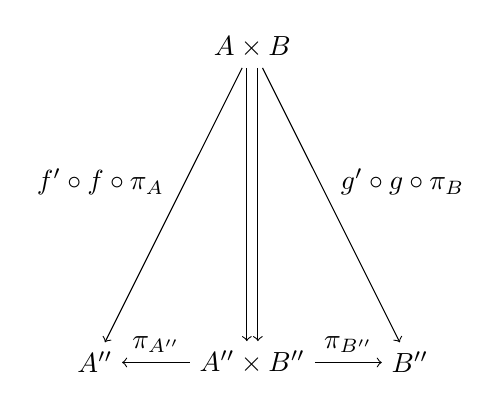
\begin{tikzpicture}[auto]
				\node (a'') at (0, -4) {$A''$};
				\node (ab) at (2, 0) {$A\times B$};
				\node (ab'') at (2, -4) {$A''\times B''$};
				\node (b'') at (4, -4) {$B''$};
				\draw[->] (ab) to node[swap]{$f'\circ f\circ\pi_A$}(a'');
				\draw[->] (ab) to node{$g'\circ g\circ\pi_B$}(b'');
				\draw[->] (ab'') to node[swap]{$\pi_{A''}$}(a'');
				\draw[->] (ab'') to node{$\pi_{B''}$}(b'');
				\draw[->,transform canvas={xshift=2pt}] (ab) to (ab'');
				\draw[->,transform canvas={xshift=-2pt}] (ab) to (ab'');
			\end{tikzpicture}
		\end{center}
	\end{proof}
	射の積を並列での合成とみなすならば、射の合成は直列での合成を表し、積と合成の交換はどちらの合成を先に計算しても結果が変わらないことを表す。

	\begin{prop}[積の一意性]
		$A$と$B$の積$A\times B$に対して、同様に$A$と$B$の積である対象$P$と射影射$\mor{\rho_A}{P}{A}$、$\mor{\rho_B}{P}{B}$が存在するとき、$A\times B\cong P$が成り立つ。またこの時、積は同型を除いて一意と呼ぶことがある。
	\end{prop}
	\begin{proof}
		積$A\times B$において、(4)の対$(X,\{f,g\})$に$(P,\{\rho_A,\rho_B\})$を当てはめると積の図式になる。よって射の対$\tuple{\rho_A,\rho_B}$が存在する。

		逆に積$P$において(4)の対$(X,\{f,g\})$に$(A\times B,\{\pi_A,\pi_B\})$を当てはめると積の図式になる。よって射の対$\tuple{\pi_A,\pi_B}$が存在する。
		\begin{center}
			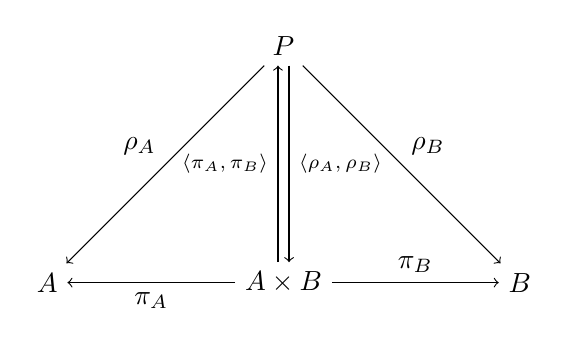
\begin{tikzpicture}[auto]
				\node (a) at (0, 0) {$A$};
				\node (ab) at (3, 0) {$A\times B$};
				\node (b) at (6, 0) {$B$};
				\node (p) at (3, 3) {$P$};
				\draw[->] (p) to node[swap]{$\rho_A$}(a);
				\draw[->] (p) to node{$\rho_B$}(b);
				\draw[->,transform canvas={xshift=2pt}] (p) to node{\scriptsize{$\tuple{\rho_A,\rho_B}$}}(ab);
				\draw[->,transform canvas={xshift=-2pt}] (ab) to node{\scriptsize{$\tuple{\pi_A,\pi_B}$}}(p);
				\draw[->] (ab) to node{$\pi_A$}(a);
				\draw[->] (ab) to node{$\pi_B$}(b);
			\end{tikzpicture}
		\end{center}
		ここで、射$\mor{\tuple{\rho_A,\rho_B}\circ\tuple{\pi_A,\pi_B}}{A\times B}{A\times B}$を射の対とする積の図式を考える、つまり積$A\times B$において対$(X,\{f,g\})$に$(A\times B,\{\pi_A,\pi_B\})$を当てはめると二つの射の対の可換性からこの積図式も可換になり、射$\tuple{\rho_A,\rho_B}\circ\tuple{\pi_A,\pi_B}$は実際に射の対になる。ここで恒等射$\mor{id_{A\times B}}{A\times B}{A\times B}$は同様に積図式を可換にするから$id_{A\times B}$もまた射の対になる。

		\begin{center}
			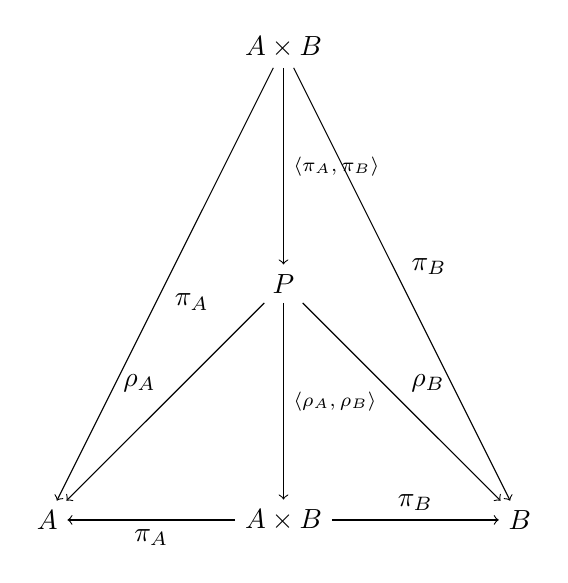
\begin{tikzpicture}[auto]
				\node (a) at (0, 0) {$A$};
				\node (ab) at (3, 0) {$A\times B$};
				\node (ab2) at (3, 6) {$A\times B$};
				\node (b) at (6, 0) {$B$};
				\node (p) at (3, 3) {$P$};
				\draw[->] (p) to node[swap]{$\rho_A$}(a);
				\draw[->] (p) to node{$\rho_B$}(b);
				\draw[->] (p) to node{\scriptsize{$\tuple{\rho_A,\rho_B}$}}(ab);
				\draw[->] (ab2) to node{\scriptsize{$\tuple{\pi_A,\pi_B}$}}(p);
				\draw[->] (ab) to node{$\pi_A$}(a);
				\draw[->] (ab) to node{$\pi_B$}(b);
				\draw[->] (ab2) to node{$\pi_A$}(a);
				\draw[->] (ab2) to node{$\pi_B$}(b);
			\end{tikzpicture}
			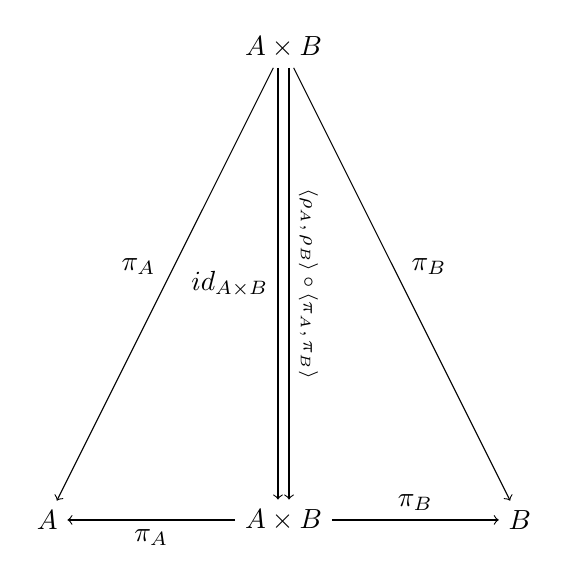
\begin{tikzpicture}[auto]
				\node (a) at (0, 0) {$A$};
				\node (ab) at (3, 0) {$A\times B$};
				\node (b) at (6, 0) {$B$};
				\node (ab2) at (3, 6) {$A\times B$};
				\draw[->] (ab2) to node[swap]{$\pi_A$}(a);
				\draw[->] (ab2) to node{$\pi_B$}(b);
				\draw[->,transform canvas={xshift=2pt}] (ab2) to node[sloped]{\scriptsize{$\tuple{\rho_A,\rho_B}\circ\tuple{\pi_A,\pi_B}$}}(ab);
				\draw[->,transform canvas={xshift=-2pt}] (ab2) to node[swap]{$id_{A\times B}$}(ab);
				\draw[->] (ab) to node{$\pi_A$}(a);
				\draw[->] (ab) to node{$\pi_B$}(b);
			\end{tikzpicture}
		\end{center}

			$\pi_A$、$\pi_B$に対する射の対は一意に定まるから$\tuple{\rho_A,\rho_B}\circ\tuple{\pi_A,\pi_B}=id_{A\times B}$が成り立つ。

			同様に射$\mor{\tuple{\pi_A,\pi_B}\circ\tuple{\rho_A,\rho_B}}{P}{P}$を射の対とする積の図式を考えると、$\tuple{\pi_A,\pi_B}\circ\tuple{\rho_A,\rho_B}=id_{P}$が成り立つ。
			すると$\tuple{\pi_A,\pi_B}$と$\tuple{\rho_A,\rho_B}$はそれぞれ同型射になり、同型射の存在が示せたので$A\times B\cong P$を示せた。
	\end{proof}
	\subsection{終対象}
	\begin{define}[終対象]
		ある圏$\cat{C}$に終対象が存在するとは、ある対象$1$が存在して圏$\cat{C}$の任意の対象$X$に対し射$\mor{!_X}{X}{1}$が一意に存在するときである。
	\end{define}
	普遍性の一般化に基づいて改めて定義してみると、
	\begin{itemize}
		\item (1)
		図式$\cat{D}$として、射と対象が一つも含まれない空圏$\cat{0}$を当てはめる。空圏は圏の公理を満たせるほどの射も対象も存在しないが、公理に違反しないため圏とみなせる。また、積を構成する図式と違って、圏$\cat{C}$の図式としての空圏は一通りしかない。
		\item (2)
		対$(U,(\tau_A)_{A\in D})$に$(1,{})$を当てはめる。図式中に対象が存在しないため、各対象への射は考慮しなくてよい。
		\item (3)
		図式に射が含まれないので無条件で可換性が成り立つ。
		\item (4)
		対$(X,(\phi_A)_{A\in D})$も(2)と同様に$(X,{})$と表せる。射の可換性どころか各対象への射の存在すら必要ないので、圏$\cat{C}$に含まれるすべての対象$X$における対を考えることができる。
		\item (5)
		終対象$1$から$X$への射$\mor{!_X}{X}{1}$が一意に定まる。同様に図式中に射が存在しないため可換性は成り立たない。
	\end{itemize}
	積の普遍性によって一意に定まる射である射の対は、与えられた図式$\cat{D}$の対象$A,B$や、$U$から図式の各対象への射$\pi_A,\pi_B$、$X$から図式の各対象への射$f,g$などの複数の対象や射によって決定されるが、終対象では与えられた図式は圏$\cat{C}$において一意に定まるし、$U$から各対象への射と$X$から各対象への射も考慮されないため一意に定まる。
	そのため射の一意性は無条件で成り立つ。

	まずは積でも示したように終対象を元を用いて調べてみる。
	\begin{prop}[終対象から終対象への射]
		終対象から終対象への射は恒等射ただ一つである。
	\end{prop}
	\begin{proof}
		終対象$1$に対して、対$(X,{})$に$(1,{})$を当てはめて考えると、$\mor{!_1}{1}{1}$は無条件で一意に定まる。
		すべての対象に恒等射は存在するから、$id_1=!_1$となり、一意に定まる。
	\end{proof}
	終対象から終対象の射を終対象の元とみなすと、終対象は元がただ一つしかない対象であると分かる。

	\begin{prop}[終対象の一意性]
		終対象$1$に対して別の終対象$1'$が存在するとき、$1\cong 1'$が成り立つ。
	\end{prop}
	\begin{proof}
		終対象$1$における$1'$からの一意に定まる射$\mor{!_1}{1'}{1}$と終対象$1'$における$1$からの一意に定まる射$\mor{{!_1}'}{1}{1'}$の合成$\mor{!_1\circ {!_1}'}{1}{1}$と$\mor{{!_1}'\circ!_1}{1'}{1'}$はそれぞれ終対象から終対象への射である。

		よって$!_1\circ {!_1}'=id_1$と${!_1}'\circ!_1=id_1'$が成り立ち、$!_1$、${!_1}'$が同型射になるから$1\cong 1'$が成り立つ。
	\end{proof}

	\subsection{演習問題}
	\begin{enumerate}
		\item 積$A\times B$において、$\tuple{\pi_A,\pi_B}=id_{A\times B}$を示せ。
		\item 対象$A,B$と終対象$1$において、任意の射$\mor{f}{A}{B}$に対して$!_B\circ f=!_A$が成り立つことを示せ。
		\item $A\times 1\cong A$を示せ。(Hint: $\pi_A$と$\tuple{id_A,!_X}$が同型射であることを示せばよい)
	\end{enumerate}
	\section{関手}
	\section{自然変換}
	\section{随伴関手}
	\section{デカルト閉圏}
	\section{米田の補題}

	\begin{thebibliography}{99}
	\bibitem{1} S.マックレーン, (2019)『圏論の基礎』(三好博之・高木理訳)丸善出版
	\bibitem{2} Steve Awodey, (2016)『圏論-原書第2版』(前原和寿訳)共立出版
	\bibitem{3} 壱大整域 \url{http://alg-d.com/math/kan_extension/}
	\bibitem{4} nLab \url{https://ncatlab.org/nlab/show/HomePage}
	\bibitem{5} Category Theory for Programmers: The Preface \url{https://bartoszmilewski.com/2014/10/28/category-theory-for-programmers-the-preface/}
	\end{thebibliography}


\end{document}
